\subsection{UML2-Komponentendiagramm}
\begin{center}
	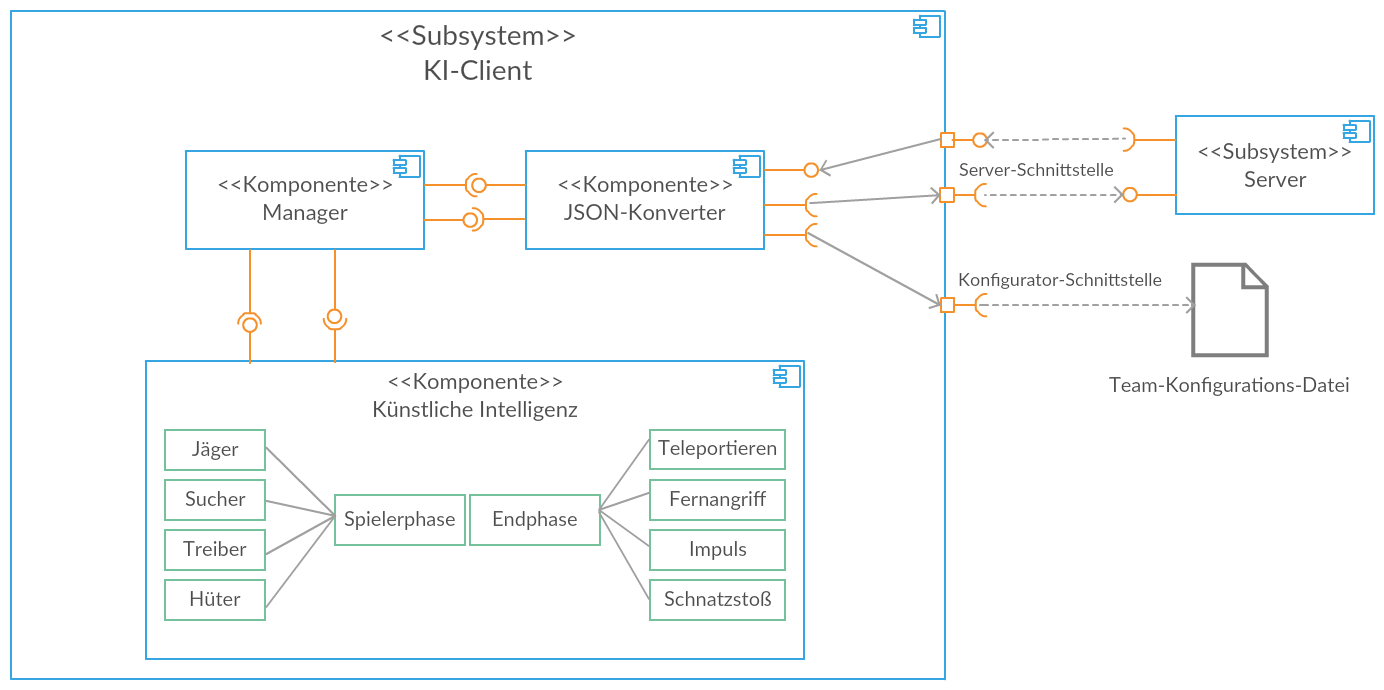
\includegraphics[width=16cm]{images/KI-Komponenten.png}
\end{center}

\subsection{Beschreibungen}
\begin{description}
	\item[KI-Client:] 
	Das Subsystem KI-Client ist eine Kommandozeilenanwendung, die sich wie ein Nutzer-Client mit einem Server verbindet, einer Partie beitritt und, gesteuert von einer KI, einen menschlichen Spieler simuliert. 
	\\
	\item[Manager:]
	Diese Komponente verwaltet die Daten des KI-Client, insbesondere die aktuelle Spielsituation und verarbeitet die Anwendungsparameter.\\ Der Manager empfängt vom JSON-Parser die aktuelle Spielsituation und aktualisiert seine gespeicherten Daten entsprechend. Er übergibt seine Daten an die KI, damit diese Entscheidungen über die durchzuführenden Aktionen treffen kann. Anschließend empfängt er die Entscheidungen der KI und aktualisiert die gespeicherte Spielsituation entsprechend, bevor er sie dem JSON-Parser übergibt.\\
	Zu Beginn einer Partie erhält der Manager vom JSON-Parser die Daten aus der zu verwendende Team-Konfigurationsdatei. \\
	Der Manager ist die zentrale Komponente des Subsystems und behandelt den Programmverlauf und die Parameter, damit die KI sich ausschließlich mit dem Entscheiden befassen kann.
	\\
	\item[JSON-Parser:]
	Diese Komponente fungiert als Dolmetscher für die Kommunikation zwischen KI-Client, Server und Team-Konfigurator.\\
	Der JSON-Parser empfängt die vom Kommunikator kommenden Nachrichten im JSON-Format und extrahiert daraus Daten über die aktuelle Spielsituation, die er anschließend dem Manager übergibt. Andersherum empfängt er Daten vom Manager, verpackt sie in einer Nachricht im JSON-Format und sendet sie an den Kommunikator.\\
	Außerdem liest der JSON-Parser Team-Konfigurationsdateien, extrahiert die Daten und gibt sie an den Manager weiter.\\
	Das Übersetzen der JSON-Dateien wird in eine eigene Komponente ausgelagert, damit der Manager unabhängig von den Konventionen der JSON-Nachrichten ist und das Subsystem leicht an diese angepasst werden kann.
	\\
	\item[Künstliche Intelligenz] 
	Diese Komponente trifft Entscheidungen über durchzuführende Aktionen anhand der aktuellen Spielsituation.\\
	Die künstliche Intelligenz, kurz KI, empfängt Daten vom Manager und verarbeitet sie in ihrer jeweiligen Logik, um die nächste durchzuführende Aktion zu ermitteln. Sobald sie eine Entscheidung getroffen hat, teilt sie diese dem Manager zur weiteren Verarbeitung mit.\\
	Die interne Struktur der künstlichen Intelligenz enthält eine Logik für jede Spielfiguren-Rolle und jede mögliche Einmischung, da jede Spielfigur anhand ihrer Aufgabe und Spezialisierung handeln muss.\\
	Die KI soll dabei unabhängig von den anderen Komponenten sein, damit sie problemlos zu jedem Zeitpunkt optimiert und für unterschiedliche Schwierigkeitsstufen ausgetauscht werden kann.
	\\
	\item[Kommunikator]
	Diese Komponente ist dafür zuständig, mit dem Server zu kommunizieren.\\
	Der Kommunikator stellt eine Verbindung mit dem angegebenen Server her, hält sie aufrecht und versucht, sie bei Verbindungsabbruch wiederherzustellen. Er empfängt Nachrichten vom Server und gibt sie unverarbeitet an den JSON-Parser weiter und überträgt umgekehrt die vom JSON-Parser kommenden Daten an den Server.\\
	Diese Funktionen werden von einer separaten Komponente übernommen, da sie in anderen Subsystemen ebenfalls gebraucht werden und der Kommunikator dort wiederverwendet werden kann. 
\end{description}

\subsection{Zuordnung der Funktionalen Anforderungen}

Die funktionalen Anforderungen gemäß dem Pflichtenheft werden den Komponenten folgendermaßen zugeteilt:

\begin{center}
	\begin{tabular}{|l|l|}
		\hline
		\textbf{Komponente} & \textbf{Abgedeckte funktionale Anforderungen}\\\hline
		Manager & FA1 - FA8\\
		& FA10 - FA20\\
		& FA44 - FA47\\
		& FA73 - FA75\\\hline
		JSON-Parser & FA54\\\hline
		Künstliche Intelligenz & FA17 - FA 21\\
		& FA26 - FA28\\
		& FA30 - FA35\\
		& FA37 - FA42\\
		&FA46 - FA47\\
		&FA50\\\hline
		Kommunikator & FA55\\\hline
		
	\end{tabular}
\end{center}
